% ch-ref-domain.tex -- reference: root keys, Grid, Initial, Substrate, Fluid
\chapter{Grid, initial state, substrate and fluid}
\label{ch:ref-domain}

This chapter documents the four blocks that describe \emph{what} is being
computed: the mesh and the domain (\key{Grid}), the state the run starts from
(\key{Initial}), the shape of the solid underneath the film
(\key{Substrate}), and the liquid's material properties (\key{Fluid}). It also
covers the handful of keys that live at root level, outside any block. The
physics terms, the boundary conditions and the numerical settings are in
\cref{ch:ref-physics,ch:ref-bcout,ch:ref-numerics}.

Every default, type and range quoted here is the one the parser actually
applies. Where a key is marked \reqd{}, omitting it terminates the run. A
range written as \emph{range $[a:b]$}, or a bound written as \emph{at least},
is checked when the file is read, and a value outside it stops the run; words
such as \emph{positive} or \emph{non-zero} say what makes sense and are not
checked. These tables are held to the parser by \file{tools/doc\_keys.py},
which \code{ctest} runs (\code{doc\_keys}).

\section{Root level}
\label{sec:ref-domain:root}

Keys written at the top of the file, before the first table header, identify
the run and choose the horizontal length scale. \key{SolverName} is a version gate,
not a solver selector: the model is chosen by \key{Physics.ConcField.Model}
together with \key{Grid.Dimension}. \key{JobName} names the result directory
created next to the run; the input file is copied into it and the ParaView
index file is named after it.

\begin{keytable}{Keys at root level\label{tab:root-keys}}\key{SolverName} & string & \reqd & Solver and input-format stamp. Must be exactly \val{"Yuzen-1.0"}; any other string aborts the run. It names the \code{MAJOR.MINOR} series only, so a patch release does not change it (\cref{ch:policy}). \\
\key{JobName} & string & \reqd & Name of the result directory. Any string. \\
\key{LengthScaleType} & string & \val{"capillary"} & How the horizontal length scale $L_0$ is chosen. \val{"capillary"} gives $L_0=\sqrt{\sigma_0/(\rho g)}$; \val{"custom"} takes $L_0$ from \key{LengthScale}. \\
\key{LengthScale} & double & \val{1.0} & Horizontal length scale in meters, read unconditionally but used only when \key{LengthScaleType} is \val{"custom"}. Positive in practice. \\
\key{InputFormatVersion} & string & \val{"1.0"} & Version of the input format the file was written for. When present it must be \val{"1.0"}, the only format this version reads (\cref{sec:ref-numerics:formatversion}). \\
\end{keytable}

No case in \file{cases/} sets either length-scale key, so every shipped case
runs on the capillary length.

\section{\key{Grid}}
\label{sec:ref-domain:grid}

\key{Grid} is required and must appear exactly once; a duplicate aborts the
run. It fixes the dimensionality of the problem, the number of interior cells
and the physical extent of the domain. Two ghost layers per side are added
internally, so the arrays the solver allocates are larger than \key{Nx} and
\key{Ny} suggest.

\begin{keytable}{Keys of \key{Grid}\label{tab:grid-keys}}\key{Dimension} & string & \reqd & \val{"xh"} = one horizontal direction (a 1-D film), \val{"xyh"} = two. With \key{Physics.ConcField.Model} it selects the solver model. \\
\key{Nx} & int & \reqd & Cells along $x$, range $[1:1000000]$. \\
\key{Ny} & int & \val{1} & Cells along $y$, range $[1:1000000]$. Must be $\ge 2$ when \key{Dimension} is \val{"xyh"}. With \val{"xh"} the film is one-dimensional and \key{Ny} is not used; the \val{"CZ"} model, which reads it, resets it to 1 with a warning if it was set to anything else. \\
\key{Nz} & int & \val{1} & Cells through the film thickness, range $[1:1000000]$. Used only by the \val{"CZ"} model, which requires $\mathrm{Nz}\ge 2$; ignored by every well-mixed model. \\
\key{Xmin} & double & \reqd & Lower $x$ bound of the domain, in meters. \\
\key{Xmax} & double & \reqd & Upper $x$ bound, in meters; must exceed \key{Xmin}. The cell width is $(\mathrm{Xmax}-\mathrm{Xmin})/\mathrm{Nx}$. \\
\key{Ymin} & double & \val{0} & Lower $y$ bound, in meters. Read but not used when \key{Dimension} is \val{"xh"}. \\
\key{Ymax} & double & \val{1} & Upper $y$ bound, in meters. Read but not used when \key{Dimension} is \val{"xh"}. \\
\end{keytable}

\begin{note}[There is a cap on the total, not just on each axis]
  Each axis is capped at one million cells, but the product is capped as well:
  $(\mathrm{Nx}+4)(\mathrm{Ny}+4)(\mathrm{Nz}+4)$ must not exceed
  $5\times10^{7}$, and a file that asks for more is rejected with a range
  error. The reason is that the grid's linear index is an \code{int}; the cap
  keeps it well inside that type. Memory is the other limit: a well-mixed
  $1024^{2}$ film needs about \SI{4}{\giga\byte}, so the cap in 2-D (some
  $10^{7}$ cells) corresponds to about \SI{40}{\giga\byte}. A step needs about \SI{4}{\kilo\byte} per cell in 2-D, \SI{2}{\kilo\byte}
  in 1-D and \SI{2}{\kilo\byte} per cell of $\mathrm{Nx}\,\mathrm{Ny}\,\mathrm{Nz}$
  in \val{"CZ"} (\cref{sec:verification:long}).
\end{note}

\begin{note}[Unused $y$ bounds are not an error]
  In a \val{"xh"} run the $y$ bounds are parsed and then ignored, so a file
  can carry leftover values from a 2-D version of the same case without any
  complaint. \file{cases/allphys\_1d\_reg.toml} does exactly this, with
  \key{Ymin} $=-1$ and \key{Ymax} $=1$ meter. Do not read such values as a
  statement about the domain.
\end{note}

\section{\key{Initial}}
\label{sec:ref-domain:initial}

\key{Initial} is required, appears exactly once, and carries no keys of its
own: it is a container for \key{Concentration} and \key{SurfaceShape}, both of
which are themselves required. Together they define the film at $t=0$ --- or,
when \key{Restart.Enable} is true, the state that the restart file replaces.

\subsection{\key{Initial.Concentration}}

\begin{keytable}{Keys of \key{Initial.Concentration}\label{tab:initial-conc-keys}}\key{Value} & double & \reqd & Initial solute (resin) concentration as a mass fraction, range $[0:1]$, written into every cell. \\
\key{Type} & string & \val{"uniform"} & Shape of the initial concentration field. The candidate list has the single member \val{"uniform"}, so any other string aborts. \\
\end{keytable}

\subsection{\key{Initial.SurfaceShape}}

This block sets the thickness scale of the whole problem and the precursor
film, and contains the shape blocks that build the profile.

\begin{keytable}{Keys of \key{Initial.SurfaceShape}\label{tab:initial-shape-keys}}\key{TotalHeight} & double & \val{1} & Film thickness scale $h_0$ in meters, positive. Every shape below is a dimensionless multiplier of it, and the whole non-dimensionalization ($T_0$, $\As$, $\Ev$, $\Df$, $\Spn$) is built from it. \\
\key{PrecursorRatio} & double & \val{0} & Precursor thickness as a fraction of \key{TotalHeight}, the dimensionless ratio $\Hstar$; in practice in $[0:1)$. Must be $>0$ when \key{Physics.DisjoiningPressure.Enable} is true, otherwise the run aborts. A non-zero value also switches on the thin-film correction of the evaporation rate. \\
\end{keytable}

The profile is assembled as
\[
  h = \mathrm{TotalHeight}\,\bigl(\text{shape}\cdot(1-\Hstar) + \Hstar\bigr),
\]
from which the substrate profile is subtracted, with a floor at
$\hstar = \Hstar\cdot\mathrm{TotalHeight}$ so that the film never thins below the
precursor.

\subsection{The seven shapes}
\label{sec:ref-domain:shapes}

Seven shape blocks are accepted inside \key{Initial.SurfaceShape}, and
\textbf{each may be repeated any number of times}, zero included. They are
drawn in \cref{fig:shapes-1d}. Look at that figure before you read the
formulas: the subsections below give each shape's definition and its keys, but
the quickest way to choose between a \key{SmoothConvex} and a
\key{MexicanHat}, or to see that \key{FlatPlane} is a tilted plane rather than
a step, is to look at the picture.

\begin{figure}[tbp]
  \centering
  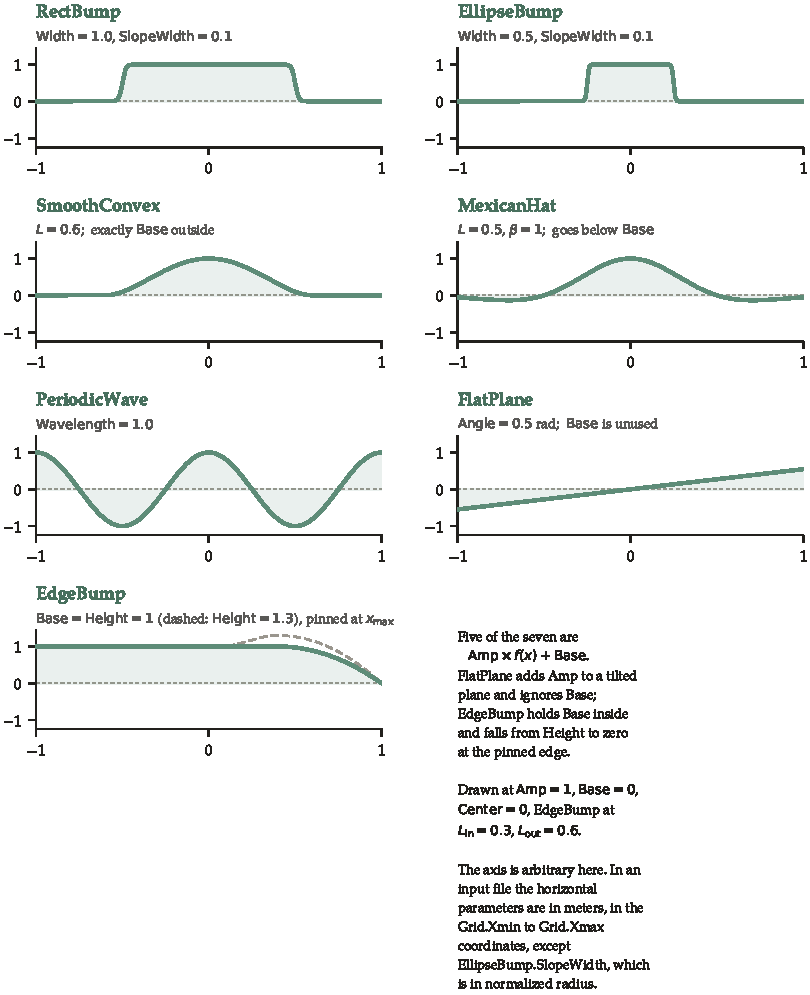
\includegraphics[width=\textwidth]{figures/shapes-1d.pdf}
  \caption{The seven shape functions, each drawn in one dimension at
    $\mathrm{Amp}=1$, $\mathrm{Base}=0$ and $\mathrm{Center}=0$ --- except
    \key{EdgeBump}, drawn as it is meant to be used, flat at
    $\mathrm{Base}=\mathrm{Height}=1$ and pinned at $x_{\max}$. Five of them
    are evaluated as $\mathrm{Amp}\times f + \mathrm{Base}$, where
    $\mathrm{Amp}$ is the block's \key{Height} --- \key{Amplitude} in
    \key{PeriodicWave} --- and $f$ is the curve drawn here; both are
    dimensionless multipliers of the container's \key{TotalHeight}. Two are
    not: \key{FlatPlane} \emph{adds} $\mathrm{Amp}$ to a tilted plane and
    ignores \key{Base} altogether, and \key{EdgeBump} holds \key{Base}
    inside and falls from \key{Height} to zero at the edge. The horizontal axis is
    arbitrary in this figure; in an input file \key{Center}, \key{Width},
    \key{Wavelength}, \key{Phase}, \key{InnerLength} and \key{OuterLength} are in meters, in
    the same coordinates as \key{Grid.Xmin} and \key{Grid.Xmax}, while
    \key{EllipseBump}'s \key{SlopeWidth} is in units of the normalized radius.
    \key{EdgeBump}'s $r_s$ is not an input key: it is derived from the domain
    edge as $x_{\max}-\key{OuterLength}$, and the panel is drawn that way. Produced by
    \file{docs/manual/\bk figures/\bk make\_shapes.py} from the definitions in
    \file{yuzen/src/\bk commonFunctions/\bk ShapeFunctions.cpp}.
    \label{fig:shapes-1d}}
\end{figure}

\subsection{How shapes combine}
\label{sec:ref-domain:createtype}

All shapes of one container are sorted by \key{Order} ascending --- ties keep
their relative order in the file --- and then applied left to right to a
running value that \textbf{starts at zero}:

\begin{description}
  \item[\val{"add"}] $\text{value} \leftarrow \max(\text{value}, \text{shape})$
    --- a \emph{union}, not a sum;
  \item[\val{"remove"}] $\text{value} \leftarrow \min(\text{value}, \text{shape})$;
  \item[\val{"stack"}] $\text{value} \leftarrow \text{value} + \text{shape}$.
\end{description}

\begin{warn}[\val{"add"} is a maximum, not an addition]
  Two overlapping bumps of height \val{0.5} combined with \val{"add"} give a
  region of height \val{0.5}, not \val{1.0}. Only \val{"stack"} adds. The
  default is \val{"add"}, so a file that lists several shapes without setting
  \key{CreateType} builds their envelope. Use \val{"add"} to place shapes side
  by side, \val{"remove"} --- a minimum --- to carve a silhouette out of what
  is already there, and \val{"stack"} to superimpose, for instance a small
  ripple on a large dome.
\end{warn}

\Cref{fig:shapes-createtype} shows the three rules applied to the same pair of
overlapping domes.

\begin{figure}[tbp]
  \centering
  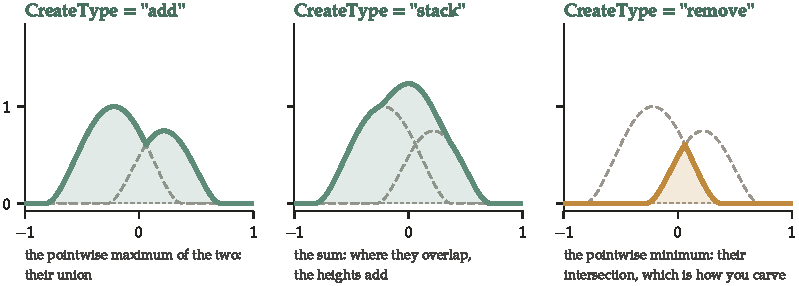
\includegraphics[width=\textwidth]{figures/shapes-createtype.pdf}
  \caption{The three merge rules of \key{CreateType}, applied to the same two
    overlapping \key{SmoothConvex} shapes (dashed). The accumulator starts at
    zero and each shape is folded into it in \key{Order}: \val{"add"} takes the
    pointwise \emph{maximum}, so it is a union and not a sum; \val{"stack"}
    takes the \emph{sum}, so overlapping heights add; \val{"remove"} takes the
    pointwise \emph{minimum}, which is how a silhouette is carved out of what
    is already there. Because the accumulator starts at zero, a shape merged
    with \val{"remove"} before anything has been added leaves nothing behind
    wherever it is positive.
    \label{fig:shapes-createtype}}
\end{figure}

Horizontal quantities --- \key{Center}, \key{Width}, \key{Wavelength},
\key{Phase}, \key{InnerLength} and \key{OuterLength}, and \key{RectBump}'s \key{SlopeWidth}
--- are in meters, in the same coordinates as \key{Grid.Xmin} and
\key{Grid.Xmax}, independently of \key{LengthScaleType}. \key{EllipseBump}'s
\key{SlopeWidth} is the exception: it softens the rim in units of the
normalized radius, so it is dimensionless. Vertical quantities --- \key{Base}, \key{Height} and
\key{Amplitude} --- are dimensionless multipliers of the container's
\key{TotalHeight}. Every \key{Center}, \key{Width}, \key{Wavelength},
\key{Phase} and \key{Angle} is an array whose length must be exactly~2, in 1-D
runs as well. A 1-D film is the line $y = 0$ of the plane the shapes are
defined in, so the $y$ components do enter: with the $y$ component of
\key{Center} and \key{Phase} at 0, as in every shipped case, each shape gives
the profile of its $x$ keys, but a bump centered further from $y = 0$ than its
$y$ extent contributes nothing, and a \key{FlatPlane} tilted in $y$ adds
$-\mathrm{Center}_y \tan \mathrm{Angle}_y$.

\subsection{\key{Initial.SurfaceShape.RectBump}}

A rectangle of height \key{Height} standing on the level \key{Base}, with
edges softened by a sigmoid so that the profile stays differentiable --- the
first panel of \cref{fig:shapes-1d}. The softening is what keeps the fourth
derivative in the height equation finite at the corners.

\begin{keytable}{Keys of \key{RectBump} (in \key{Initial.SurfaceShape} or \key{Substrate})\label{tab:shape-rectbump}}\key{Order} & int & \val{0} & Sort key; shapes are applied in ascending order. Any value. \\
\key{CreateType} & string & \val{"add"} & Merge rule: \val{"add"}, \val{"remove"} or \val{"stack"}. \\
\key{Base} & double & \val{0} & Offset added to the shape everywhere, as a fraction of \key{TotalHeight}. \\
\key{Height} & double & \val{1} & Amplitude of the bump, as a fraction of \key{TotalHeight}. \\
\key{Center} & array & \val{[0, 0]} & Center $(x,y)$ of the rectangle in meters. Length exactly~2. \\
\key{Width} & array & \val{[1, 1]} & Full width $(x,y)$ of the flat top in meters, positive. Length exactly~2. \\
\key{SlopeWidth} & array & \val{[0.05, 0.05]} & Edge-softening length $(x,y)$ in meters; internally multiplied by 0.1 to give the sigmoid width. Length exactly~2. \\
\end{keytable}

\subsection{\key{Initial.SurfaceShape.EllipseBump}}

An elliptical bump --- a flat-topped plateau with a soft rim, as the second
panel of \cref{fig:shapes-1d} shows in cross-section. The support is the
interior of $\sqrt{((x-c_x)/W_x)^2 + ((y-c_y)/W_y)^2} < 0.5$, so \key{Width}
is the \emph{full} axis length, not the semi-axis. This is the only shape any
shipped case uses.

\begin{keytable}{Keys of \key{EllipseBump} (in \key{Initial.SurfaceShape} or \key{Substrate})\label{tab:shape-ellipsebump}}\key{Order} & int & \val{0} & Sort key. \\
\key{CreateType} & string & \val{"add"} & Merge rule: \val{"add"}, \val{"remove"} or \val{"stack"}. \\
\key{Base} & double & \val{0} & Vertical offset, as a fraction of \key{TotalHeight}. \\
\key{Height} & double & \val{1} & Amplitude, as a fraction of \key{TotalHeight}. \\
\key{Center} & array & \val{[0, 0]} & Center $(x,y)$ in meters. Length exactly~2. \\
\key{Width} & array & \val{[1, 1]} & Full axes $(x,y)$ in meters, non-zero. Length exactly~2. \\
\key{SlopeWidth} & double & \val{0.05} & Edge softening of the elliptical rim, in units of the normalized radius --- a \textbf{scalar}, unlike in \key{RectBump}. \\
\end{keytable}

\begin{warn}[Work out how wide the rim actually is, in cells]
  \key{SlopeWidth} here multiplies the \emph{normalized} radius, so the width
  of the rim on the ground depends on \key{Width} as well. The profile goes
  from a tenth of \key{Height} to nine tenths of it over
  \begin{equation*}
    \Delta x \;=\; \tfrac{1}{10}\ln 81 \;\key{SlopeWidth}\,W_x
              \;\approx\; 0.44\,\key{SlopeWidth}\,W_x ,
  \end{equation*}
  and what matters is that against the cell size
  $(X_{\max}-X_{\min})/N_x$. The default \val{0.05} on a
  \SI{0.4}{\milli\metre} bump gives \SI{8.8}{\micro\metre}, half a cell on a
  60-point millimeter:
  \textbf{the default is a step on a typical mesh}, and a value written as
  though it were a length --- \val{0.1e-3}, say --- is a vertical wall.
  A wall is not merely inelegant. In \file{concz\_2d} it cuts the time step
  by a factor of 10, puts a spurious bulge of liquid in the corner
  (\SI{7.92}{\micro\metre} of film against \SI{6.05}{\micro\metre}), and
  inflates the surface excess of the concentration by a factor of 2.7. Aim for the rim to span
  several cells and check the first \file{field00000.dat} before trusting a
  long run.
\end{warn}

\subsection{\key{Initial.SurfaceShape.PeriodicWave}}

A product of cosines about the mean level \key{Base},
\[
  \text{shape} = \mathrm{Base} + \mathrm{Amplitude}\,
    \cos\!\left(\frac{2\pi (x-x_0)}{\lambda_x}\right)
    \cos\!\left(\frac{2\pi (y-y_0)}{\lambda_y}\right),
\]
useful for a corrugated substrate or for a single wavelength of a leveling
test. It is the one shape that is not localized: it fills the whole domain, and
it is as far below \key{Base} as above it (\cref{fig:shapes-1d}).

\begin{keytable}{Keys of \key{PeriodicWave} (in \key{Initial.SurfaceShape} or \key{Substrate})\label{tab:shape-periodicwave}}\key{Order} & int & \val{0} & Sort key. \\
\key{CreateType} & string & \val{"add"} & Merge rule: \val{"add"}, \val{"remove"} or \val{"stack"}. \\
\key{Base} & double & \val{0} & Mean level of the wave, as a fraction of \key{TotalHeight}. \\
\key{Amplitude} & double & \val{1} & Amplitude, as a fraction of \key{TotalHeight}. \\
\key{Wavelength} & array & \val{[1, 1]} & Wavelengths $(\lambda_x,\lambda_y)$ in meters, non-zero. Length exactly~2. \\
\key{Phase} & array & \val{[0, 0]} & Phase as a \textbf{spatial offset} $(x_0,y_0)$ in meters, not as an angle. Length exactly~2. \\
\end{keytable}

\subsection{\key{Initial.SurfaceShape.FlatPlane}}

A tilted plane,
\[
  \text{shape} = (x-c_x)\tan\alpha_x + (y-c_y)\tan\alpha_y + \mathrm{Height},
\]
that is, height \key{Height} at \key{Center} and a constant slope away from
it, as in \cref{fig:shapes-1d}. Combined with \val{"stack"} it adds a uniform
wedge to any other shape.

\begin{keytable}{Keys of \key{FlatPlane} (in \key{Initial.SurfaceShape} or \key{Substrate})\label{tab:shape-flatplane}}\key{Order} & int & \val{0} & Sort key. \\
\key{CreateType} & string & \val{"add"} & Merge rule: \val{"add"}, \val{"remove"} or \val{"stack"}. \\
\key{Height} & double & \val{1} & Height of the plane at \key{Center}, as a fraction of \key{TotalHeight}. \\
\key{Center} & array & \val{[0, 0]} & Pivot $(x,y)$ in meters about which the plane is tilted. Length exactly~2. \\
\key{Angle} & array & \val{[0, 0]} & Tilt about $x$ and $y$, in \textbf{radians}. Length exactly~2. \\
\end{keytable}

\key{FlatPlane} has \textbf{no} \key{Base} key: its constructor is always
called with a base of zero. Writing one has no effect, and no warning.

\begin{warn}[The two angles in the file are in different units]
  \key{FlatPlane.Angle} is in radians, like every other angle in the input
  file. \key{Physics.DisjoiningPressure.ContactAngle} is the single exception:
  it is in \emph{degrees}, and is range-checked against $[0:90]$. A contact
  angle written as \val{0.17} is therefore not $10^\circ$ but a sixth of a
  degree.
\end{warn}

\subsection{\key{Initial.SurfaceShape.MexicanHat}}

The Ricker wavelet: a central peak surrounded by a circular trough. Unlike the
other localized shapes it dips \emph{below} \key{Base} around its peak, and it
never quite returns to it, which \cref{fig:shapes-1d} makes plain at a glance:
\[
  \text{shape} = \mathrm{Base} + \mathrm{Height}\,(1-r^2)\,e^{-\beta r^2},
  \qquad
  r^2 = \left(\frac{x-c_x}{L_x}\right)^{2} + \left(\frac{y-c_y}{L_y}\right)^{2}.
\]

\begin{keytable}{Keys of \key{MexicanHat} (in \key{Initial.SurfaceShape} or \key{Substrate})\label{tab:shape-mexicanhat}}\key{Order} & int & \val{0} & Sort key. \\
\key{CreateType} & string & \val{"add"} & Merge rule: \val{"add"}, \val{"remove"} or \val{"stack"}. \\
\key{Base} & double & \val{0} & Vertical offset, as a fraction of \key{TotalHeight}. \\
\key{Height} & double & \val{1} & Amplitude, as a fraction of \key{TotalHeight}. \\
\key{Center} & array & \val{[0, 0]} & Center $(x,y)$ in meters. Length exactly~2. \\
\key{Width} & array & \val{[1, 1]} & Radial scales $(L_x,L_y)$ in meters. Length exactly~2; a zero component makes the shape vanish everywhere. \\
\key{Beta} & double & \val{1} & Decay $\beta$ of the Gaussian envelope, non-dimensional; non-negative in practice. \\
\end{keytable}

\subsection{\key{Initial.SurfaceShape.SmoothConvex}}

A compact dome, $\mathrm{Height}\,(1-r^2)^2$ inside $r\le 1$ and exactly
\key{Base} outside it, with $r$ defined as for \key{MexicanHat}. Unlike an
ellipsoid it meets the surrounding level with zero slope, so it introduces no
curvature spike at its rim; compare its shoulders with those of
\key{MexicanHat} in \cref{fig:shapes-1d}.

\begin{keytable}{Keys of \key{SmoothConvex} (in \key{Initial.SurfaceShape} or \key{Substrate})\label{tab:shape-smoothconvex}}\key{Order} & int & \val{0} & Sort key. \\
\key{CreateType} & string & \val{"add"} & Merge rule: \val{"add"}, \val{"remove"} or \val{"stack"}. \\
\key{Base} & double & \val{0} & Level outside the support, returned verbatim for $r>1$, as a fraction of \key{TotalHeight}. \\
\key{Height} & double & \val{1} & Peak amplitude, as a fraction of \key{TotalHeight}. \\
\key{Center} & array & \val{[0, 0]} & Center $(x,y)$ in meters. Length exactly~2. \\
\key{Width} & array & \val{[1, 1]} & Radial half-extents $(L_x,L_y)$ in meters, non-zero. Length exactly~2. \\
\end{keytable}

\subsection{\key{Initial.SurfaceShape.EdgeBump}}

The film against a pinned edge: flat at \key{Base} inside the domain, it falls
to zero at the edge over the last \key{OuterLength} --- the last panel of
\cref{fig:shapes-1d}. It exists to start a run from a film that is already
pinned at a wall, with a meniscus, instead of from a discontinuity. With $p$
the distance from the switch-over point $r_s$, which lies \key{OuterLength}
inside the edge, positive toward the edge, the profile is
%
\begin{equation}
  f(p) = \bigl(1-\sigma(p)\bigr)\Bigl[(H-B)\,\bigl(1-p^2/L_i^2\bigr)\,e^{-p^2/(\alpha L_i^2)} + B\Bigr]
       + \sigma(p)\,H\,\bigl(1 - p^2/L_o^2\bigr),
\end{equation}
%
with $B$ = \key{Base}, $H$ = \key{Height}, $L_i$ = \key{InnerLength}, $L_o$ =
\key{OuterLength}, $\alpha$ = \key{Alpha} and $\sigma$ a logistic step of width
$0.1\,L_i$ at $r_s$. \textbf{The usual setting is $\mathrm{Height} =
\mathrm{Base}$} (for a film of uniform thickness, both 1): the film is flat up
to $r_s$ and falls as a parabola to zero at the edge. A \key{Height} above
\key{Base} raises a rim at $r_s$ (the dashed curve of the figure), one below it
a dip.

\textbf{\key{EdgeBump} exists only inside \key{Initial.SurfaceShape}}; the
\key{Substrate} block does not accept it.

\begin{keytable}{Keys of \key{Initial.SurfaceShape.EdgeBump}\label{tab:shape-edgebump}}\key{Order} & int & \val{0} & Sort key. \\
\key{CreateType} & string & \val{"add"} & Merge rule: \val{"add"}, \val{"remove"} or \val{"stack"}. \\
\key{Base} & double & \val{0} & Level of the film inside the domain, away from the edge, as a fraction of \key{TotalHeight}. \\
\key{Height} & double & \val{1} & Level at the switch-over point \key{OuterLength} inside the edge, from which the film falls to zero at the edge; equal to \key{Base} for a film flat up to the meniscus. \\
\key{Location} & string & \val{"Xmax"} & Which domain edge the bump is attached to: \val{"Xmin"}, \val{"Xmax"}, \val{"Ymin"} or \val{"Ymax"}. The matching \key{Boundary} block must be of type \val{"Pinning"}. \\
\key{Alpha} & double & \val{1} & Width parameter $\alpha>0$ of the inner Gaussian $\exp(-(1/\alpha)(p/\mathrm{InnerLength})^2)$, non-dimensional. \\
\key{InnerLength} & double & \val{1} & Inner length scale in meters, positive; also sets the blending width, $0.1\,\mathrm{InnerLength}$. \\
\key{OuterLength} & double & \val{1} & Width of the meniscus in meters: the distance from the edge to the switch-over point, over which the film falls to zero. \\
\end{keytable}

A pinned edge needs a film that reaches zero there, and \key{EdgeBump} is the
shape that provides one: its profile falls to zero at the wall whatever
\key{Base} and \key{Height} are, which with a small \key{PrecursorRatio} leaves only the precursor. The
solver checks the result before the first step (\cref{sec:ref-bcout:boundary}).

\begin{note}[\key{Location} and the boundary condition must agree]
  \code{CheckParameters} rejects the input unless the
  \key{Boundary.<Location>BC.Type} matching every \key{EdgeBump} is
  \val{"Pinning"}, with the message \code{Input mismatch}. It is one of the
  cross-key constraints checked before the model is built; that the film then
  reaches zero at the pinned edge is checked just before the first step
  (\cref{sec:ref-bcout:boundary}).
\end{note}

\section{\key{Substrate}}
\label{sec:ref-domain:substrate}

\key{Substrate} is optional and may appear at most once. It describes the
solid surface $s(x,y)$ that the film sits on. The substrate never moves and
never changes. It enters the capillary-pressure and vertical-gravity terms
through the free-surface height $h+s$, so \textbf{if neither of those two terms
is enabled the substrate shape does nothing at all}
(\cref{sec:terms:laplace,sec:terms:vgravity}).

If the block is absent the substrate is flat: no shape is registered and the
profile is never evaluated.

\begin{keytable}{Keys of \key{Substrate}\label{tab:substrate-keys}}\key{TotalHeight} & double & \val{1} & Height scale of the topography in meters; the profile is \key{TotalHeight} times the combined shape. Independent of \key{Initial.SurfaceShape.TotalHeight}. \\
\end{keytable}

\key{Substrate} accepts the same repeatable shape blocks as
\key{Initial.SurfaceShape} \textbf{except \key{EdgeBump}} --- that is,
\key{RectBump}, \key{EllipseBump}, \key{PeriodicWave}, \key{FlatPlane},
\key{MexicanHat} and \key{SmoothConvex} --- with identical key names, types,
defaults, ranges and units. The two parsers are the same code writing into a
different destination, so \cref{tab:shape-rectbump,tab:shape-ellipsebump,tab:shape-periodicwave,tab:shape-flatplane,tab:shape-mexicanhat,tab:shape-smoothconvex}
apply unchanged. The only other difference is that \key{Base}, \key{Height}
and \key{Amplitude} are fractions of \key{Substrate.TotalHeight} here.

\begin{note}[The substrate ordering path is untested]
  No case in \file{cases/} sets \key{Order} inside a \key{Substrate} shape
  block, and no case uses any substrate shape other than \key{EllipseBump}.
  If you build a substrate from several shapes, check the result in the first
  field output before trusting it.
\end{note}

\section{\key{Fluid}}
\label{sec:ref-domain:fluid}

\key{Fluid} is required and appears exactly once. It has one key of its own,
and five sub-blocks that are \textbf{all required} --- a missing one aborts the
run --- even though every key inside them has a default.

\begin{keytable}{Keys of \key{Fluid}\label{tab:fluid-keys}}\key{Name} & string & \val{"CR-EX"} & Label for the liquid. Recorded and printed in the log only; it selects no property set. \\
\end{keytable}

\subsection{Concentration dependence}
\label{sec:ref-domain:fluidconc}

Three of the five sub-blocks give a property at a reference concentration and
the way it varies around it. These three laws are what the \key{BaseValue},
\key{BaseConc}, \key{Coef} and \key{Exponent} keys mean:

\begin{align}
  \sigma(c) &= \mathrm{BaseValue} + \mathrm{Coef}\,(c - \mathrm{BaseConc}),
    \label{eq:fluid-sigma}\\
  \mu(c)    &= \mathrm{BaseValue}\,
    \exp\bigl(\mathrm{Exponent}\,(c - \mathrm{BaseConc})\bigr),
    \label{eq:fluid-mu}\\
  D(c)      &= \mathrm{BaseValue}\,
    \exp\bigl(\mathrm{Exponent}\,(c - \mathrm{BaseConc})\bigr).
    \label{eq:fluid-diff}
\end{align}

Surface tension is linear in concentration; viscosity and diffusivity are
exponential. \Cref{eq:fluid-mu} is the strongest non-linearity in the solver:
with \key{Exponent} near 10, a concentration change of 0.1 multiplies the
viscosity by $e$, and it is this that stops the flow as the film dries.
\Cref{eq:fluid-sigma} feeds two different places --- the slope \key{Coef} is
the Marangoni number $\Ma$, and $\sigma(c)$ also enters the mobility of the
capillary-pressure term, so drying changes how fast the film levels
(\cref{ch:concentration}).

\subsection{\key{Fluid.Density}}

\begin{keytable}{Keys of \key{Fluid.Density}\label{tab:fluid-density-keys}}\key{Value} & double & \val{1070} & Liquid density $\rho$ in \si{\kilogram\per\metre\cubed}, positive. Assumed independent of concentration. Enters the capillary length $L_0$, and the groups $\Bo$, $\Pvec$ and $\Spn$. \\
\end{keytable}

\subsection{\key{Fluid.SurfaceTension}}

\begin{keytable}{Keys of \key{Fluid.SurfaceTension}, see \cref{eq:fluid-sigma}\label{tab:fluid-surften-keys}}\key{BaseValue} & double & \val{0.028} & Surface tension $\sigma_0$ at \key{BaseConc}, in \si{\newton\per\metre}, positive. Sets the capillary length and the time scale. \\
\key{BaseConc} & double & \val{0.5} & Reference concentration of the linear law, mass fraction in $[0:1]$. \\
\key{Coef} & double & \val{0.014} & $\mathrm{d}\sigma/\mathrm{d}c$ in \si{\newton\per\metre} per unit concentration; the sign matters. Its ratio to \key{BaseValue} is the Marangoni number $\Ma$. Forced to zero when \key{Physics.SolutoCapillarity.Enable} is false. \\
\end{keytable}

\subsection{\key{Fluid.Viscosity}}

\begin{keytable}{Keys of \key{Fluid.Viscosity}, see \cref{eq:fluid-mu}\label{tab:fluid-visc-keys}}\key{BaseValue} & double & \val{0.115} & Viscosity $\mu_0$ at \key{BaseConc}, in \si{\pascal\second}, positive. Sets the time scale $T_0 = \mu_0 L_0^4/(\sigma_0 h_0^3)$. \\
\key{BaseConc} & double & \val{0.5} & Reference concentration, mass fraction in $[0:1]$. \\
\key{Exponent} & double & \val{8} & Exponential rate, non-dimensional, any value. A realistic figure is about 10, i.e.\ $\Delta c = 0.1$ multiplies $\mu$ by $e$. \\
\end{keytable}

\subsection{\key{Fluid.Diffusivity}}

\begin{keytable}{Keys of \key{Fluid.Diffusivity}, see \cref{eq:fluid-diff}\label{tab:fluid-diff-keys}}\key{BaseValue} & double & \val{9.78e-11} & Solute diffusivity $D_0$ at \key{BaseConc}, in \si{\metre\squared\per\second}, positive. Enters $\Pen = E_0 h_0/D_0$ and $\Df = D_0 T_0/L_0^2$. \\
\key{BaseConc} & double & \val{0.5} & Reference concentration, mass fraction in $[0:1]$. \\
\key{Exponent} & double & \val{6.94} & Exponential rate, non-dimensional, any value; usually negative in practice. \\
\end{keytable}

\subsection{\key{Fluid.MolarMass}}

Only the ratio $\Mr = \mathrm{Resin}/\mathrm{Solvent}$ is used, in Raoult's law
for the evaporation rate (\cref{sec:terms:evaporation}), so any consistent
pair of units will do.

\begin{keytable}{Keys of \key{Fluid.MolarMass}\label{tab:fluid-molar-keys}}\key{Solvent} & double & \val{106} & Molar mass of the solvent, positive; \si{\gram\per\mole} in practice, but any unit consistent with \key{Resin}. \\
\key{Resin} & double & \val{2200} & Molar mass of the solute, positive, in the same unit as \key{Solvent}. \\
\end{keytable}
